\section{Privacy and the collection of personal data}

A few years ago in Minneapolis an angry man walked into a retail store called \textit{Target} and demanded to see the manager. \textit{"My daughter got this in the mail!"} he exclaimed, showing some coupons in his hand. \textit{"She is still in high school, and you're sending her coupons for baby clothes and cribs? Are you trying to encourage her to get pregnant?"} \cite{youtube01} \cite{nytimes01} The coupons were indeed addressed to the man's daughter and contained advertisements for maternity clothing, nursery furniture and pictures of smiling infants. The manager apologized, and called a few days later to apologize again.

On the phone, though, the father was somewhat abashed. \textit{"I had a talk with my daughter"}. he said. \textit{"It turns out there has been some activities in my house I haven't been completely aware of. She's due in August. I owe you an apology."} \cite{nytimes01} But how did the retail store know that the girl is pregnant before her own father? As a matter of fact \textit{Target} was observing the purchasing habits of its customers through their membership cards. In this case, a change like purchasing scent-free lotions and soap, extra-big bags of cotton balls, hand sanitizers, washcloths and supplements containing calcium magnesium and zinc indicated a likely pregnancy to the retail store's cleverly constructed advertising algorithm. In fact, the algorithm was so advanced, that it could even predict the due date with a relatively small time window so that the store can send coupons timed to very specific stages of pregnancy.

In our modern age data is power. Data is now a commodity -- arguably the world's most valuable commodity, dethroning oil from its former number one position. \cite{economist01} Big software companies have recognized this a long time ago and offer convenient, easy to use software and services \textit{"for free}." In reality however, nothing is free. Users of these services are paying with their personal data, ranging from simple personal identifiers to more complex usage statistics and metrics. This data is most often cross-referenced with other similarly collected databases to draw conclusions and offer a more personalized user experience -- including advertisements.

As a result, we are now subject to a greater level of surveillance than in any point in history, and we hand over most of our data willingly. \cite{factortech01} It can be expected, that the increasing amount of \textit{internet-of-things} devices and the introduction of \textit{5G networking} will result in an even bigger surge in the amount and types of data collected.

\section{Regulation}
Even the Big Tech companies (who not surprisingly are also the biggest collectors and consumers of personal data) are
beginning to acknowledge that personal data collection needs to be regulated. \cite{wired01} Recent privacy scandals of Google (Google+) \cite{precursor01}, Facebook, Cambridge Analytica \cite{wiki01}, Amazon \cite{wiki02} and others \cite{technadu01} seem to support the importance of the need for a stricter regulation as well.

More recently governments are slowly catching up on the regulation front. One prime example is the \textit{"General Data Protection Regulation" (GDPR)} of the European Union. The \textit{GDPR} got some critique \cite{clearcritique,thomsonreuters}, but it has a solid foundation. It regulates how the collection of personal data is disclosed to the data subjects, and demands that data stored on people in the EU undergo either an \textbf{\textit{anonymization}} or a \textbf{\textit{pseudonymization}} process. \cite{wiki03, wiki04} The main difference between the two processes is, that pseudonymized data can be restored to its original state by re-adding identifiers, while anonymized data can not be restored. In this document we will mostly be discussing anonymization, however it is not hard to imagine how one would construct a pseudonymization algorithm given a working anonymization algorithm.

\section{Data anonymization}
In the previous chapters we briefly introduced the sociological and political aspects of privacy. Now we will proceed to discuss the concept of \textbf{\textit{anonymization}} and its technical aspects. So how exactly can we define anonymization?

\paragraph{Definition} \textsc{Data anonymization} has been defined as a process by which personal data is irreversibly altered in such a way that a data subject can no longer be identified directly or indirectly, either by the data controller alone or in collaboration with any other party. \cite{wiki04, iso01}

A typical \textit{data controller} can be a hospital storing medical data about its patients. The data is then released to third parties or government entities, for example to draw conclusions in an epidemic outbreak. We can see, that some parts of the data like address, age, race, gender -- although personal -- can be necessary to draw accurate statistical conclusions. To allow the extraction of useful statistics while also protecting the privacy of its patients, the hospital will need to alter the data before handing it over.

\section{k-anonymity}

\subsection{Insufficiency of identifier truncation} \label{sec:insuff}

Before diving into the definition of k-anonymity, let's take the previous example a little bit further, and consider the following patient data taken from the hospital's database:

\begin{figure}[H]
	\centering
	\begin{tabular}{|c|l|c|l|l|c|l|}
		\hline
		\textbf{SSN} & \textbf{Name} & \textbf{Age} & \textbf{Race} & \textbf{Gender} & \textbf{Zip Code} & \textbf{Disease} \\
		\hline
		1001 & John Smith  & 34 & White & Male   & 18500 & Flu \\
		1002 & Eva Brown   & 27 & Asian & Female & 18200 & Cancer \\
		1003 & Anne Parker & 17 & White & Female & 18500 & Hypertension \\
		1004 & Mark Wayne  & 34 & Black & Male   & 18200 & Flu \\
		\hline
	\end{tabular}
	\caption{Example patient data}
	\label{fig:example-patient-data}
\end{figure}

In order to attempt to remove personal information from the data, one -- albeit naïve -- approach the hospital could choose is to simply \textit{truncate} all fields that contain identifiers. In the above example they will be the \textit{social security number} and \textit{name} fields. The resulting table will look something like this:

\begin{figure}[H]
	\centering
	\begin{tabular}{|c|l|l|c|l|}
		\hline
		\textbf{Age} & \textbf{Race} & \textbf{Gender} & \textbf{Zip Code} & \textbf{Disease} \\
		\hline
		34 & White & Male   & 18500 & Flu \\
		27 & Asian & Female & 18200 & Cancer \\
		17 & White & Female & 18500 & Hypertension \\
		34 & Black & Male   & 18200 & Flu \\
		\hline
	\end{tabular}
	\caption{Truncated patient data}
	\label{fig:truncated-patient-data}
\end{figure}

Unfortunately by using an external public database -- for example census records or a phone book -- an attacker could still piece together which person was diagnosed with which disease, thus rendering the hospital's data protection method useless. This is called a \textbf{\textit{table join attack}}:

\begin{figure}[H]
	\centering
	\begin{tabular}{|c|l|c|}
		\hline
		\textbf{Age} & \textbf{Name} & \textbf{Zip Code} \\
		\hline
		34 & John Smith  & 18500 \\
		27 & Eva Brown   & 18200 \\
		17 & Anne Parker & 18500 \\
		34 & Mark Wayne  & 18200 \\
		\hline
	\end{tabular}
	\caption{Census data}
	\label{fig:census-data}
\end{figure}

\begin{figure}[H]
	\centering
	\begin{tabular}{|l|c|l|l|c|l|}
		\hline
		\textbf{Name} & \color{red}{\textbf{Age}} & \textbf{Race} & \textbf{Gender} & \color{red}{\textbf{Zip Code}} & \textbf{Disease} \\
		\hline
		John Smith  & \color{red}{34} & White & Male   & \color{red}{18500} & Flu \\
		Eva Brown   & \color{red}{27} & Asian & Female & \color{red}{18200} & Cancer \\
		Anne Parker & \color{red}{17} & White & Female & \color{red}{18500} & Hypertension \\
		Mark Wayne  & \color{red}{34} & Black & Male   & \color{red}{18200} & Flu \\
		\hline
	\end{tabular}
	\caption{Patient data restored with join attack}
	\label{fig:joined-patient-data}
\end{figure}

One might think, that this does not usually happen outside of fabricated examples. Unfortunately, as Sweeney observed \cite{sweeney} for 87\% of the U.S. population the combination of date of birth, gender and zip code corresponded to a unique person \cite{aggarwal} -- which could easily make the above example reality.

\subsection{Data model} \label{sec:data_model}

Most anonymization algorithms work on data tables with a concrete \textit{schema} so we will adopt this model as well. Tables can also be viewed as \textit{n} row vectors, or \textit{tuples}. Each tuple represents an individual piece of data, and consists of \textit{m} attributes \((c_1, c_2, \cdots, c_m)\). Attributes are sometimes also referred to as \textit{dimensions}.

\subsubsection{Attribute types}

\paragraph{identifiers:} these attributes by themselves alone can be used to identify the person whom the data belongs to without the need to reference any other attributes. It is easy to see, that anonymization algorithms will always need to truncate or suppress all of these attributes from the final anonymized data set.

\paragraph{quasi-identifiers:} as illustrated by the examples in section \ref{sec:insuff} some attributes are not identifiers themselves but can still be used in conjunction with external data sources to identify the concrete person. These attributes are \textit{quasi-identifier} attributes, and will be subject to some level of generalization or suppression based on the algorithm being used (refer to the next section called \textit{"Data hiding techniques"} for a more precise explanation of generalization and suppression).

\paragraph{non-identifiers:} attributes, which the \textit{data controller} deems irrelevant in the context of anonymization are non-identifiers. We can often extract useful statistics from their values, but they are meaningless without pairing them with additional attributes.

\subsubsection{Data hiding techniques} In order to remove sensitive data from a database, anonymization algorithms use common data hiding techniques. In this section we will briefly introduce two commonly used, and illustrate how they work on simple examples.

\paragraph{suppression} is very similar to truncating all sensitive data values. When looking at a single attribute (like age) in a database, truncating it would redact \textit{all} values. Suppression on the other hand redacts \textit{some} of the values, while retaining the rest. \cite{aggarwal} Which values are suppressed and which values are retained is decided by the anonymization algorithm, which considers several different factors.

The following example shows the anonymization of a table using suppression only, along the quasi-identifiers Name, Age and Gender:

\begin{figure}[H]
	\centering
	\begin{tabular}{|l|c|l|c|}
		\hline
		\textbf{Name} & \textbf{Age} & \textbf{Gender} & \textbf{Salary} \\
		\hline
		John & 25 & Male   & 50000 \\
		Mark & 30 & Male   & 65000 \\
		Jill & 24 & Female & 45000 \\
		Jane & 24 & Female & 70000 \\
		\hline
	\end{tabular}
	\quad
	\begin{tabular}{|l|c|l|c|}
		\hline
		\textbf{Name} & \textbf{Age} & \textbf{Gender} & \textbf{Salary} \\
		\hline
		* & *  & Male   & 50000 \\
		* & *  & Male   & 65000 \\
		* & 24 & Female & 45000 \\
		* & 24 & Female & 70000 \\
		\hline
	\end{tabular}
	\caption{Suppression}
	\label{fig:suppression1}
\end{figure}

\paragraph{generalization} replaces values with less specific, but semantically consistent values from the same domain. For example a date can be made more generic by omitting the days and even more so by reducing it to the year only. (Note, that suppression is basically a special case of generalization -- we can create a special generalization function, which maps every value to a suppressed value in one step.)

The following example shows the anonymization of a table using generalization along the quasi-identifiers Name, Age and Gender:

\begin{figure}[H]
	\centering
	\begin{tabular}{|l|c|l|c|}
		\hline
		\textbf{Name} & \textbf{Age} & \textbf{Gender} & \textbf{Salary} \\
		\hline
		John & 25 & Male   & 50000 \\
		Mark & 30 & Male   & 65000 \\
		Jill & 24 & Female & 45000 \\
		Jane & 24 & Female & 70000 \\
		\hline
	\end{tabular}
	\quad
	\begin{tabular}{|l|c|l|c|}
		\hline
		\textbf{Name} & \textbf{Age} & \textbf{Gender} & \textbf{Salary} \\
		\hline
		* & [20-30] & Male   & 50000 \\
		* & [20-30] & Male   & 65000 \\
		* & 24      & Female & 45000 \\
		* & 24      & Female & 70000 \\
		\hline
	\end{tabular}
	\caption{Generalization}
	\label{fig:generalization}
\end{figure}


In most cases we can assume, that for each attribute a \textit{\textbf{generalization hierarchy}} exists \cite{aggarwal}. Each level of the generalization hierarchy corresponds to a partition of the attribute domain, and a refinement over the partitions on the previous level. \cite{samarati-sweeney} On the two opposing ends of the hierarchy we have singleton sets corresponding to the lack of generalization, and a single set containing all values from the domain corresponding to the highest level of generalization.

\begin{figure}[H]
	\centering
\tikzset{every picture/.style={line width=0.75pt}} %set default line width to 0.75pt
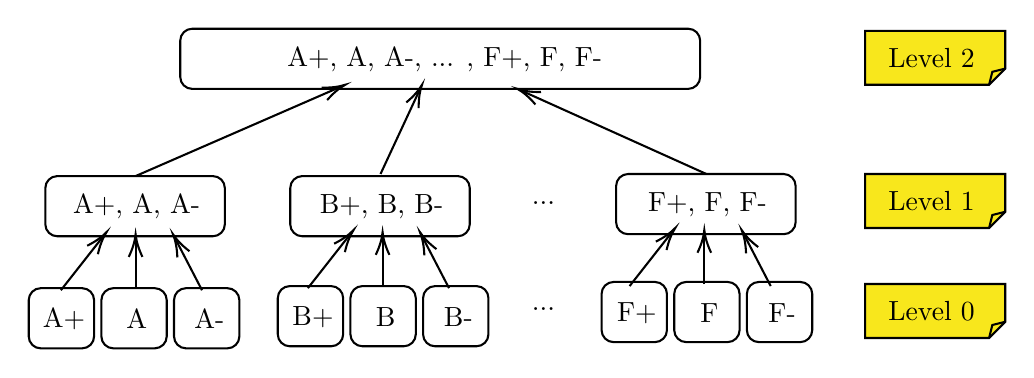
\begin{tikzpicture}[x=0.75pt,y=0.75pt,yscale=-1,xscale=1]
%uncomment if require: \path (0,457); %set diagram left start at 0, and has height of 457

%Rounded Rect [id:dp05055633926904224]
\draw   (40,265.8) .. controls (40,262.6) and (42.6,260) .. (45.8,260) -- (120.7,260) .. controls (123.9,260) and (126.5,262.6) .. (126.5,265.8) -- (126.5,283.2) .. controls (126.5,286.4) and (123.9,289) .. (120.7,289) -- (45.8,289) .. controls (42.6,289) and (40,286.4) .. (40,283.2) -- cycle ;

%Rounded Rect [id:dp15417219044870833]
\draw   (158,265.8) .. controls (158,262.6) and (160.6,260) .. (163.8,260) -- (238.7,260) .. controls (241.9,260) and (244.5,262.6) .. (244.5,265.8) -- (244.5,283.2) .. controls (244.5,286.4) and (241.9,289) .. (238.7,289) -- (163.8,289) .. controls (160.6,289) and (158,286.4) .. (158,283.2) -- cycle ;

%Rounded Rect [id:dp5566983339728413]
\draw   (315,264.8) .. controls (315,261.6) and (317.6,259) .. (320.8,259) -- (395.7,259) .. controls (398.9,259) and (401.5,261.6) .. (401.5,264.8) -- (401.5,282.2) .. controls (401.5,285.4) and (398.9,288) .. (395.7,288) -- (320.8,288) .. controls (317.6,288) and (315,285.4) .. (315,282.2) -- cycle ;

%Rounded Rect [id:dp14128108650523874]
\draw   (32,319.8) .. controls (32,316.6) and (34.6,314) .. (37.8,314) -- (57.7,314) .. controls (60.9,314) and (63.5,316.6) .. (63.5,319.8) -- (63.5,337.2) .. controls (63.5,340.4) and (60.9,343) .. (57.7,343) -- (37.8,343) .. controls (34.6,343) and (32,340.4) .. (32,337.2) -- cycle ;

%Rounded Rect [id:dp6850532710750563]
\draw   (67,319.8) .. controls (67,316.6) and (69.6,314) .. (72.8,314) -- (92.7,314) .. controls (95.9,314) and (98.5,316.6) .. (98.5,319.8) -- (98.5,337.2) .. controls (98.5,340.4) and (95.9,343) .. (92.7,343) -- (72.8,343) .. controls (69.6,343) and (67,340.4) .. (67,337.2) -- cycle ;
%Rounded Rect [id:dp49831794890726244]
\draw   (102,319.8) .. controls (102,316.6) and (104.6,314) .. (107.8,314) -- (127.7,314) .. controls (130.9,314) and (133.5,316.6) .. (133.5,319.8) -- (133.5,337.2) .. controls (133.5,340.4) and (130.9,343) .. (127.7,343) -- (107.8,343) .. controls (104.6,343) and (102,340.4) .. (102,337.2) -- cycle ;
%Rounded Rect [id:dp5034621708150937]
\draw   (152,318.8) .. controls (152,315.6) and (154.6,313) .. (157.8,313) -- (177.7,313) .. controls (180.9,313) and (183.5,315.6) .. (183.5,318.8) -- (183.5,336.2) .. controls (183.5,339.4) and (180.9,342) .. (177.7,342) -- (157.8,342) .. controls (154.6,342) and (152,339.4) .. (152,336.2) -- cycle ;
%Rounded Rect [id:dp4304422122223639]
\draw   (187,318.8) .. controls (187,315.6) and (189.6,313) .. (192.8,313) -- (212.7,313) .. controls (215.9,313) and (218.5,315.6) .. (218.5,318.8) -- (218.5,336.2) .. controls (218.5,339.4) and (215.9,342) .. (212.7,342) -- (192.8,342) .. controls (189.6,342) and (187,339.4) .. (187,336.2) -- cycle ;
%Rounded Rect [id:dp8079993361963536]
\draw   (222,318.8) .. controls (222,315.6) and (224.6,313) .. (227.8,313) -- (247.7,313) .. controls (250.9,313) and (253.5,315.6) .. (253.5,318.8) -- (253.5,336.2) .. controls (253.5,339.4) and (250.9,342) .. (247.7,342) -- (227.8,342) .. controls (224.6,342) and (222,339.4) .. (222,336.2) -- cycle ;
%Rounded Rect [id:dp3763444142614236]
\draw   (308,316.8) .. controls (308,313.6) and (310.6,311) .. (313.8,311) -- (333.7,311) .. controls (336.9,311) and (339.5,313.6) .. (339.5,316.8) -- (339.5,334.2) .. controls (339.5,337.4) and (336.9,340) .. (333.7,340) -- (313.8,340) .. controls (310.6,340) and (308,337.4) .. (308,334.2) -- cycle ;
%Rounded Rect [id:dp025410635634430356]
\draw   (343,316.8) .. controls (343,313.6) and (345.6,311) .. (348.8,311) -- (368.7,311) .. controls (371.9,311) and (374.5,313.6) .. (374.5,316.8) -- (374.5,334.2) .. controls (374.5,337.4) and (371.9,340) .. (368.7,340) -- (348.8,340) .. controls (345.6,340) and (343,337.4) .. (343,334.2) -- cycle ;
%Rounded Rect [id:dp6345478019954871]
\draw   (378,316.8) .. controls (378,313.6) and (380.6,311) .. (383.8,311) -- (403.7,311) .. controls (406.9,311) and (409.5,313.6) .. (409.5,316.8) -- (409.5,334.2) .. controls (409.5,337.4) and (406.9,340) .. (403.7,340) -- (383.8,340) .. controls (380.6,340) and (378,337.4) .. (378,334.2) -- cycle ;
%Rounded Rect [id:dp5704093284694525]
\draw   (105,194.8) .. controls (105,191.6) and (107.6,189) .. (110.8,189) -- (349.7,189) .. controls (352.9,189) and (355.5,191.6) .. (355.5,194.8) -- (355.5,212.2) .. controls (355.5,215.4) and (352.9,218) .. (349.7,218) -- (110.8,218) .. controls (107.6,218) and (105,215.4) .. (105,212.2) -- cycle ;
%Straight Lines [id:da5982931753916951]
\draw    (47.5,315) -- (68.26,288.57) ;
\draw [shift={(69.5,287)}, rotate = 488.16] [color={rgb, 255:red, 0; green, 0; blue, 0 }  ][line width=0.75]    (10.93,-3.29) .. controls (6.95,-1.4) and (3.31,-0.3) .. (0,0) .. controls (3.31,0.3) and (6.95,1.4) .. (10.93,3.29)   ;

%Straight Lines [id:da7014066905322178]
\draw    (83.5,314) -- (83.5,290) ;
\draw [shift={(83.5,288)}, rotate = 450] [color={rgb, 255:red, 0; green, 0; blue, 0 }  ][line width=0.75]    (10.93,-3.29) .. controls (6.95,-1.4) and (3.31,-0.3) .. (0,0) .. controls (3.31,0.3) and (6.95,1.4) .. (10.93,3.29)   ;

%Straight Lines [id:da7237438732675705]
\draw    (115.5,315) -- (102.42,289.78) ;
\draw [shift={(101.5,288)}, rotate = 422.59000000000003] [color={rgb, 255:red, 0; green, 0; blue, 0 }  ][line width=0.75]    (10.93,-3.29) .. controls (6.95,-1.4) and (3.31,-0.3) .. (0,0) .. controls (3.31,0.3) and (6.95,1.4) .. (10.93,3.29)   ;

%Straight Lines [id:da9667373614001253]
\draw    (166.5,314) -- (187.26,287.57) ;
\draw [shift={(188.5,286)}, rotate = 488.16] [color={rgb, 255:red, 0; green, 0; blue, 0 }  ][line width=0.75]    (10.93,-3.29) .. controls (6.95,-1.4) and (3.31,-0.3) .. (0,0) .. controls (3.31,0.3) and (6.95,1.4) .. (10.93,3.29)   ;

%Straight Lines [id:da4011582897955388]
\draw    (202.5,313) -- (202.5,289) ;
\draw [shift={(202.5,287)}, rotate = 450] [color={rgb, 255:red, 0; green, 0; blue, 0 }  ][line width=0.75]    (10.93,-3.29) .. controls (6.95,-1.4) and (3.31,-0.3) .. (0,0) .. controls (3.31,0.3) and (6.95,1.4) .. (10.93,3.29)   ;

%Straight Lines [id:da5300154790184455]
\draw    (234.5,314) -- (221.42,288.78) ;
\draw [shift={(220.5,287)}, rotate = 422.59000000000003] [color={rgb, 255:red, 0; green, 0; blue, 0 }  ][line width=0.75]    (10.93,-3.29) .. controls (6.95,-1.4) and (3.31,-0.3) .. (0,0) .. controls (3.31,0.3) and (6.95,1.4) .. (10.93,3.29)   ;

%Straight Lines [id:da49332566002225353]
\draw    (321.5,313) -- (342.26,286.57) ;
\draw [shift={(343.5,285)}, rotate = 488.16] [color={rgb, 255:red, 0; green, 0; blue, 0 }  ][line width=0.75]    (10.93,-3.29) .. controls (6.95,-1.4) and (3.31,-0.3) .. (0,0) .. controls (3.31,0.3) and (6.95,1.4) .. (10.93,3.29)   ;

%Straight Lines [id:da6387699678510084]
\draw    (357.5,312) -- (357.5,288) ;
\draw [shift={(357.5,286)}, rotate = 450] [color={rgb, 255:red, 0; green, 0; blue, 0 }  ][line width=0.75]    (10.93,-3.29) .. controls (6.95,-1.4) and (3.31,-0.3) .. (0,0) .. controls (3.31,0.3) and (6.95,1.4) .. (10.93,3.29)   ;

%Straight Lines [id:da7454255088680426]
\draw    (389.5,313) -- (376.42,287.78) ;
\draw [shift={(375.5,286)}, rotate = 422.59000000000003] [color={rgb, 255:red, 0; green, 0; blue, 0 }  ][line width=0.75]    (10.93,-3.29) .. controls (6.95,-1.4) and (3.31,-0.3) .. (0,0) .. controls (3.31,0.3) and (6.95,1.4) .. (10.93,3.29)   ;

%Straight Lines [id:da41690437548834924]
\draw    (83.5,260) -- (182.67,216.8) ;
\draw [shift={(184.5,216)}, rotate = 516.46] [color={rgb, 255:red, 0; green, 0; blue, 0 }  ][line width=0.75]    (10.93,-3.29) .. controls (6.95,-1.4) and (3.31,-0.3) .. (0,0) .. controls (3.31,0.3) and (6.95,1.4) .. (10.93,3.29)   ;

%Straight Lines [id:da9088806507789935]
\draw    (201.5,259) -- (220.66,217.81) ;
\draw [shift={(221.5,216)}, rotate = 474.94] [color={rgb, 255:red, 0; green, 0; blue, 0 }  ][line width=0.75]    (10.93,-3.29) .. controls (6.95,-1.4) and (3.31,-0.3) .. (0,0) .. controls (3.31,0.3) and (6.95,1.4) .. (10.93,3.29)   ;

%Straight Lines [id:da6354688861477524]
\draw    (358.5,259) -- (269.32,218.82) ;
\draw [shift={(267.5,218)}, rotate = 384.25] [color={rgb, 255:red, 0; green, 0; blue, 0 }  ][line width=0.75]    (10.93,-3.29) .. controls (6.95,-1.4) and (3.31,-0.3) .. (0,0) .. controls (3.31,0.3) and (6.95,1.4) .. (10.93,3.29)   ;

%Shape: Folded Corner [id:dp6484816765083135]
\draw  [fill={rgb, 255:red, 248; green, 231; blue, 28 }  ,fill opacity=1 ] (494.7,338) -- (435,338) -- (435,312) -- (502.5,312) -- (502.5,330.2) -- cycle -- (494.7,338) ; \draw   (502.5,330.2) -- (496.26,331.76) -- (494.7,338) ;
%Shape: Folded Corner [id:dp9570029764461927]
\draw  [fill={rgb, 255:red, 248; green, 231; blue, 28 }  ,fill opacity=1 ] (494.7,285) -- (435,285) -- (435,259) -- (502.5,259) -- (502.5,277.2) -- cycle -- (494.7,285) ; \draw   (502.5,277.2) -- (496.26,278.76) -- (494.7,285) ;
%Shape: Folded Corner [id:dp38314853861140774]
\draw  [fill={rgb, 255:red, 248; green, 231; blue, 28 }  ,fill opacity=1 ] (494.7,216) -- (435,216) -- (435,190) -- (502.5,190) -- (502.5,208.2) -- cycle -- (494.7,216) ; \draw   (502.5,208.2) -- (496.26,209.76) -- (494.7,216) ;

% Text Node
\draw (84,275) node  [align=left] {A+, A, A-};
% Text Node
\draw (202,275) node  [align=left] {B+, B, B-};
% Text Node
\draw (359,274) node  [align=left] {F+, F, F-};
% Text Node
\draw (280,273) node  [align=left] {...};
% Text Node
\draw (49,329) node  [align=left] {A+};
% Text Node
\draw (84,329) node  [align=left] {A};
% Text Node
\draw (119,329) node  [align=left] {A-};
% Text Node
\draw (204,328) node  [align=left] {B};
% Text Node
\draw (239,328) node  [align=left] {B-};
% Text Node
\draw (169,328) node  [align=left] {B+};
% Text Node
\draw (360,326) node  [align=left] {F};
% Text Node
\draw (395,326) node  [align=left] {F-};
% Text Node
\draw (325,326) node  [align=left] {F+};
% Text Node
\draw (280,324) node  [align=left] {...};
% Text Node
\draw (232.42,204) node  [align=left] {A+, A, A-, ... , F+, F, F-};
% Text Node
\draw (467,325) node  [align=left] {Level 0};
% Text Node
\draw (467,272) node  [align=left] {Level 1};
% Text Node
\draw (467,203) node  [align=left] {Level 2};


\end{tikzpicture}
	\caption{Generalization hierarchy for school grades}
	\label{fig:grades-hierarchy}
\end{figure}

The generalization hierarchy is a useful model, but it is not without restrictions -- especially when considering very large or infinite value domains (for example integer numbers). In later chapters we will see how we can implement more flexible generalization hierarchy for our anonymization algorithm.

\subsection{Definition of k-anonymity} \label{sec:definition_of_anonymity}

The \textit{k-anonymity} model was originally proposed by Samarati and Sweeney \cite{samarati-sweeney} \cite{sweeney02}. The idea is to generalize some of the data in the input table to ensure, that \textit{for each tuple in the anonymized table there are at least \(k-1\) other tuples in the table that are identical to it along the quasi-identifier attributes}. While achieving this, the anonymization algorithm should also minimize the \textit{cost of generalization}.

A k-anonymized data table will be "immune" to join attacks or \textit{record linkages} even if the attacker has access to all quasi-identifying attributes of all the individuals represented in the table \cite{aggarwal}. This is because each individual tuple is hidden among \(k-1\) other identical tuples. Note however that it is the responsibility of the  data controller the correctly identify all quasi-identifiers in the table and provide a sufficient generalization hierarchy for them.

Selecting an appropriate \textit{k} value is also the data controller's responsibility. While picking a large \textit{k} value will ensure a bigger level of privacy, it also reduces the amount of information left in the data set. The \textit{k} value should always be selected by considering the needs of the application.

\begin{figure}[H]
	\centering
	\small
	\begin{tabular}{|c|l|l|l|l|l|l|}
		\hline
		\textbf{Name} & \textbf{Status} & \textbf{Gender} & \textbf{Age} & \textbf{Kids} & \textbf{Income} & \textbf{Grade} \\
		\hline
		* & employee   & *      & [18..36] & [0..2] & [10000..50000] & [A] \\
		* & client     & female & [18..36] & [0..2] & [15000..15624] & [A-] \\
	    * & employee   & *      & [30]     & [2]    & [30000..39999] & [A, A+, A-] \\
	    * & employee   & *      & [18..36] & [0..2] & [10000..50000] & [A] \\
	    * & client     & male   & [18..36] & [2]    & [40000..44999] & [A, A+, A-] \\
	    * & client     & female & [18..36] & [0..2] & [15000..15624] & [A-] \\
	    * & employee   & male   & [18..36] & [2]    & [40000..44999] & [A, A+, A-] \\
		* & client     & *      & [30]     & [2]    & [30000..39999] & [A, A+, A-] \\
		\hline
	\end{tabular}
	\caption{An anonymized table for k=2 with various data types}
	\label{k-anonymized-table}
\end{figure}

Now we can formally define k-anonymity: \cite{aggarwal}:

\paragraph{Definition} \textsc{k-anonymity with suppression}: \\
given \(x_1,\cdots,x_n \in \Sigma^m\) and the anonymity parameter \textit{k}, obtain a k-anonymous suppression function \textit{t} so that \textit{c(t)} is minimized.

A \textbf{k-anonymous suppression function} \textit{t} maps each \(x_i\) to \(\bar{x_i}\) by replacing some components of \(x_i\) by \(*\), so that every \(\bar{x_i}\) is identical to at least \(k-1\) other \(\bar{x_j}\)s.

The \textbf{cost of \textit{t} suppression function} \textit{c(t)} is the total number of hidden entries (\(*s\)) in all the \(\bar{x_i}\)s.

\begin{center}
	\rule{0.9\textwidth}{0.3pt}
\end{center}

\paragraph{Definition} \textsc{k-anonymity with generalization}: \\
given \(x_1,\cdots,x_n \in \Sigma^m\) and the anonymity parameter \textit{k}, obtain a k-anonymous generalization function \textit{h} so that \textit{c(h)} is minimized.

Let the \(j^{th}\) attribute have domain \(D^j\) and \(l_j\) levels of generalization. Let the partition corresponding to the \(h^{th}\) level be denoted by \(g_{h(y)}\). A \textbf{generalization function} \textit{h} is a function that maps a pair \((i,j), i \le n, j \le m\) to a level of generalization \(h(i,j) \le l_j\).

Let \(h(x_i)\) denote the \textit{generalized} vector corresponding to \(x_i\), i.e. \[h(x_i) = (g_{h(i,1)}(x_1[1]), \cdots, g_{h(i,m)}(x_i[m])).\] \textit{h} is a \textbf{k-anonymous generalization function} if for every \(i, h(x_i)\) is identical to \(h(x_j)\) for at least \(k-1\) values of \(j \neq i\).

Consider a k-anonymous generalization function \textit{h}. It incurs a \textbf{cost} of \(r/l_j\) whenever it generalizes a value for the \(j^{th}\) attribute to the \(r^{th}\) level. The \textbf{total cost incurred by the generalization function} \textit{h} is defined as the sum of the costs incurred over all the entries of the table, i.e. \(c(h) = \Sigma_i\Sigma_jh(i,j)/l_j\).

\begin{center}
	\rule{0.9\textwidth}{0.3pt}
\end{center}

While this definition seems complicated at first, it basically just states, that we are looking for the \textit{"cheapest"} generalization (or suppression) function which partitions the rows in such a way, that at least \textit{k} identical rows are present in each partition after applying the function -- this is in-line with the rule of k-anonymity stated earlier.

The complication comes from calculating the cost incurred by the function. For a suppression function we simply need to count the number of suppressed entries. For a generalization function however we need to consider the maximum level of generalization possible for the attribute's domain, and the level of generalization applied by the function in order to find the generalization cost for a single entry. This cost for a single entry will always be a rational  number between \([0..1]\). The total cost of applying the generalization function is the sum of all of these costs.

It is also worth noting, that the problem of \textbf{k-anonymity with suppression} is a special case of the problem of \textbf{k-anonymity with generalization}. \cite{aggarwal} This can be proven by using a special generalization function which only has one level of generalization for each attribute domain which corresponds to completely hiding the element value. It can easily be seen, that this special generalization function is equivalent to a suppression function for the same \textit{k} anonymity parameter.

\subsection{NP-hardness of k-anonymity}

\paragraph{Theorem} k-anonymity with suppression is NP-hard even for a ternary alphabet (\(\Sigma = {0, 1, 2}\)). \cite{aggarwal}

The complete proof will not be presented in this document, but the core idea is, that the NP-hard problem \textit{Edge Partition Into Triangles} (Kann, 1994) can be reduced into the problem of k-anonymity with suppression for \(k=3\). \cite{aggarwal} Furthermore, by reduction from \textit{Edge Partition Into r-Cliques} (Kann, 1994) the proof can be extended to any \(k \ge 2\) integer value.

Let's pause for a moment and consider the consequences of the above theorem. A decision problem H is NP-hard, when for every problem L in NP, there is a polynomial-time reduction from L to H. \cite{leeuwen} In other words problems in this class are \textit{"at least as hard as the hardest problems in NP"}. \cite{wiki07} As a consequence if \textbf{\(P \neq NP\)}, then NP-hard problems cannot be solved in polynomial time. \cite{wiki06, wiki07}

In the next chapter we will outline a polynomial \textbf{approximation} algorithm for the k-anonymity problem. This means, that we won't always get the \textit{optimal} solution -- i.e. the cost of anonymization is not  always \textit{minimal} -- but we get one, that's "good enough".